\subsection{Import JSON Recording}
\label{sec:ui_import_json}

This task allows importing of JSON data from a previous jASTERIX run into the opened database, either from text files or from archives. \\

\begin{figure}[H]
  \hspace*{-0.5cm}
    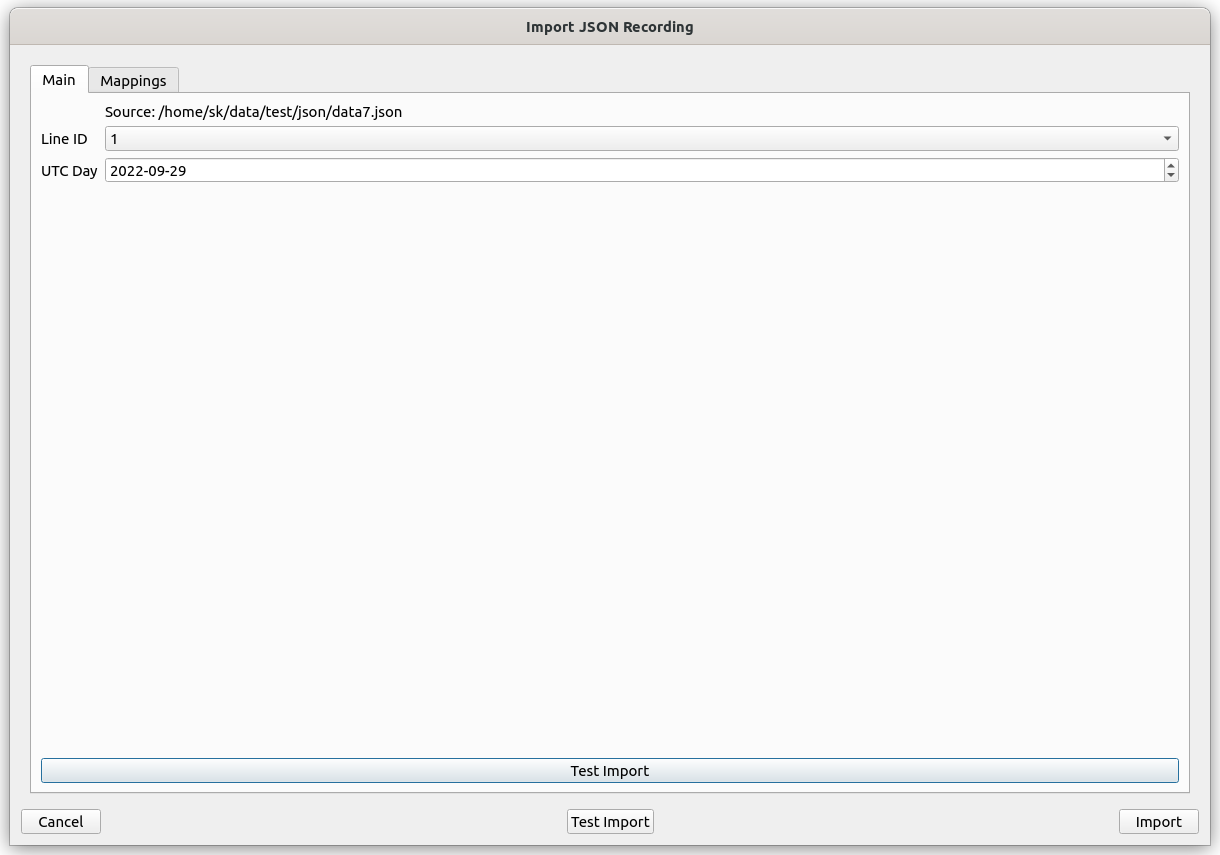
\includegraphics[width=17cm]{figures/import_json_data.png}
  \caption{Import JSON data}
\end{figure}

There exist 2 tabs:

\begin{itemize}  
\item Main: File list and support functions/parameters
\item Mappings: Defintion of created database content based on decoded data
\end{itemize}
\ \\

\subsubsection{Main Tab}

At the top, the recording file to be imported is shown. Below, there exists a combobox defining in which line the data should be written. \\

The 'Cancel' button aborts the import. Using the 'Test Import' button the import process can be tested without inserting the data into the database. 
The 'Import' button triggers the import of the selected file into into the database with the given options. This function can be run multiple times. \\

\subsubsection{Mappings Tab}

\begin{figure}[H]
    \hspace*{-0.5cm}
    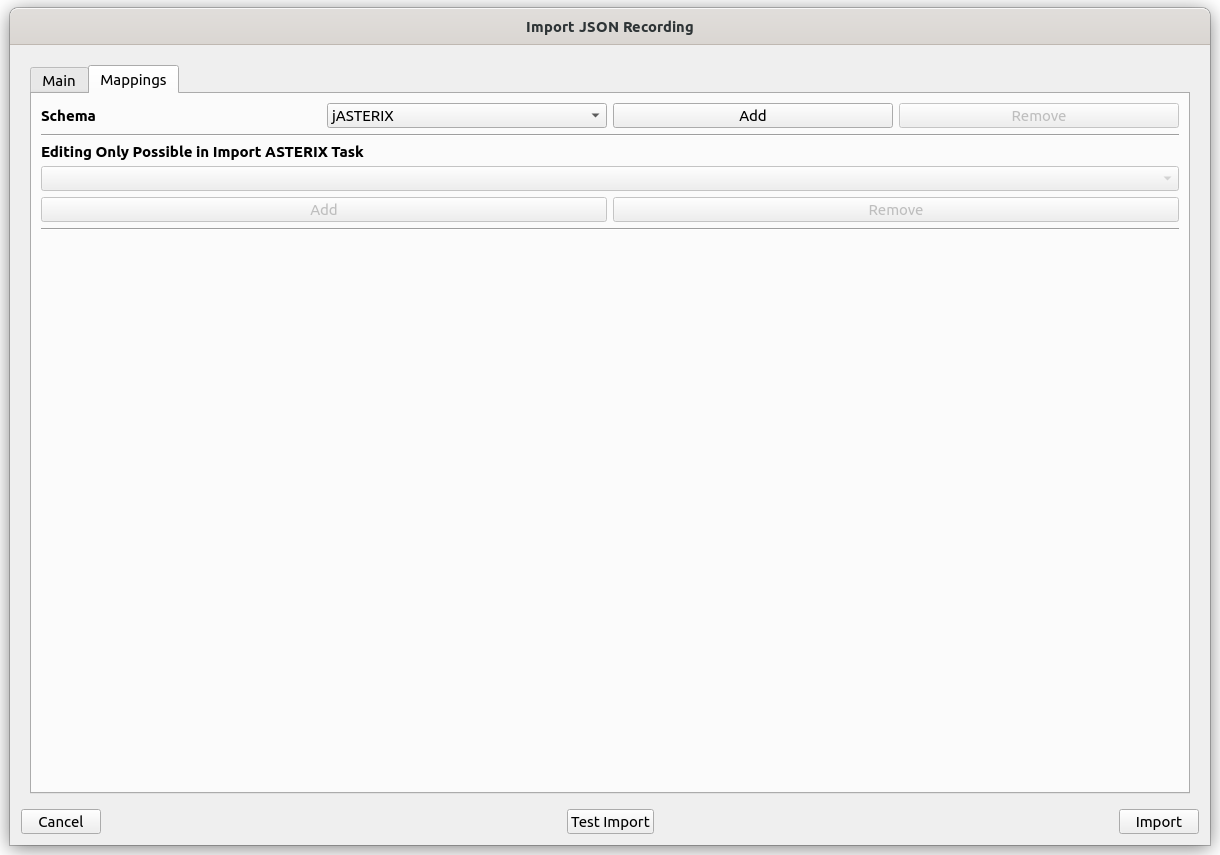
\includegraphics[width=17cm,frame]{figures/import_json_data_object_parser.png}
  \caption{Import JSON Data Object Parser}
\end{figure}

At the top, the GUI elements can be used to show/add/remove JSON objects parsers. Below that, the currently selected JSON object parser is shown and can be configured. \\

A JSON object parser in this context is the function that parses the JSON content and creates database content from it. For different supported  data type a dedicated parser defines the mapping from JSON to database content. \\

For common users normally no interaction is recommended, but it might be sometimes interesting what database content is created from which JSON data.

\paragraph{Top Elements}

Using the drop-down menu, the to-be-shown parser can be selected. The buttons allow for adding and removing JSON object parsers.

The following options exist:
\begin{itemize}  
%\item SDDL: Import JSON created by the SDDL tool (v0.2 or later)
%\item ADSBexchange: Import JSON from the ADSBexchange platform
%\item OpenSkyNetwork: Import JSON from the OpenSky Network platform
\item jASTERIX: Data previously decoded/saved with jASTERIX
\end{itemize}
\ \\

Please note that the jASTERIX mapping schema has to be edited in the 'Import ASTERIX Data' task.


% \paragraph{Parser GUI Elements}
% 
% The exact definition of how the parsing works is out of scope for this document, so only a short summy is given here. For more information please contact the author.
% 
% \begin{itemize}  
% \item JSON Object Parser Name: Named after the ASTERIX category and the DBObject to which it is mapped
% \item Variable List:
% \begin{itemize}  
% \item Active checkbox: Defines if the specific mapping is used
% \item JSON Key: JSON location and name of the data to be mapped
% \item Comment: Additional information with example values
% \item DBOVariable: Target variable to which this data is mapped
% \item Mandatory checkbox: Defines if the JSON object is skipped if the JSON key is not found
% \item Unit: Unit and dimension of the JSON data, only defined if conversion is needed
% \item Format: Special format of the JSON data, only defined if conversion is needed
% \end{itemize}
% \end{itemize}

\subsubsection{Running}

Using the 'Import' button the task can be performed. During import a status indication will be shown:

\begin{figure}[H]
  \center
    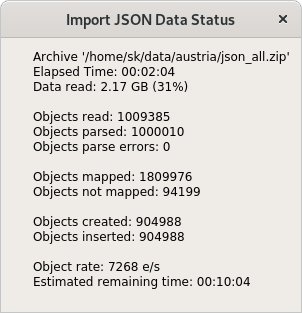
\includegraphics[width=6cm]{figures/json_import_status.png}
  \caption{Import JSON data status}
\end{figure}

If data sizes can be read from the archive (supported by ZIP but not by GZIP), predictions about the remaining time will be shown.

After import, a confirmation will be shown as follows:

\begin{figure}[H]
  \center
    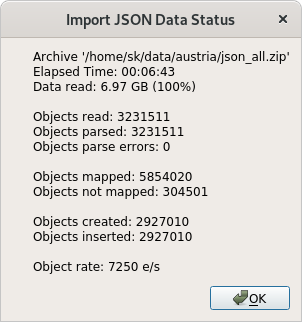
\includegraphics[width=6cm,frame]{figures/json_import_done.png}
  \caption{Import JSON data done}
\end{figure}

%\paragraph{Comments}

%Importing performance strongly depends on CPU performance (multi-threading very beneficial), but a SDDL JSON import of 3 million target reports takes about 7 minutes on the author's hardware. \\

%\includegraphics[width=0.5cm]{../../data/icons/hint.png} Please note that, since ADSBexchange JSON is not compliant to JSON standard (at least from the used test datasets), parsing errors will be shown and only a small percentage of target reports is imported.
